\problemname{Digital Circuit}

\begin{quote}
\textit{Note:} in this problem, you have to write your solution in C++.
\end{quote}

There is a circuit, which consists of $N + M$ gates numbered from $0$ to $N + M - 1$. Gates $0$ to
$N-1$ are \emph{threshold gates}, whereas gates $N$ to $N + M - 1$ are \emph{source gates}.

Each gate, except for gate $0$, is an input to exactly one threshold gate. Specifically, for each $i$
such that $1 \leq i \leq N + M - 1$, gate $i$ is an input to gate $P[i]$, where
$0 \leq P[i] \leq N-1$. Importantly, we also have $P[i] < i$. Moreover, we assume $P[0] = -1$. Each
threshold gate has one or more inputs. Source gates do not have any inputs.

Each gate has a \emph{state} which is either $0$ or $1$. The initial states of the source gates are
given by an array $A$ of $M$ integers. That is, for each $j$ such that $0 \leq j \leq M-1$, the
initial state of the source gate $N + j$ is $A[j]$.

The state of each threshold gate depends on the states of its inputs and is determined as follows.
First, each threshold gate is assigned a \emph{threshold parameter}. The parameter assigned to a
threshold gate with $c$ inputs must be an integer between $1$ and $c$ (inclusive). Then, the state of
a threshold gate with parameter $p$ is $1$, if at least $p$ of its inputs have state $1$, and $0$
otherwise.

For example, suppose there are $N = 3$ threshold gates and $M = 4$ source gates. The inputs to gate
$0$ are gates $1$ and $6$, the inputs to gate $1$ are gates $2$, $4$ and $5$, and the only input to
gate $2$ is gate $3$.

This example is illustrated in the following picture.

\begin{center}
  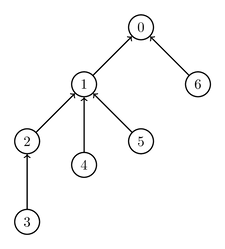
\includegraphics[width=0.30\textwidth]{circuit-tree.png}
\end{center}

Suppose that source gates $3$ and $5$ have state $1$, while source gates $4$ and $6$ have state $0$.
Assume we assign parameters $1$, $2$ and $2$ to threshold gates $2$, $1$ and $0$ respectively. In
this case, gate $2$ has state $1$, gate $1$ has state $1$ and gate $0$ has state $0$. This assignment
of parameter values and the states is illustrated in the following picture. Gates whose state is $1$
are marked in black.

\begin{center}
  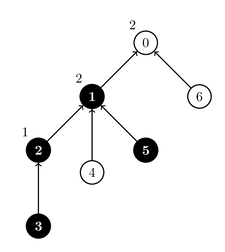
\includegraphics[width=0.30\textwidth]{circuit-states.png}
\end{center}

The states of the source gates will undergo $Q$ updates. Each update is described by two integers $L$
and $R$ ($N \leq L \leq R \leq N + M - 1$) and toggles the states of all source gates numbered
between $L$ and $R$, inclusive. That is, for each $i$ such that $L \leq i \leq R$, source gate $i$
changes its state to $1$, if its state is $0$, or to $0$, if its state is $1$. The new state of each
toggled gate remains unchanged until it is possibly toggled by one of the later updates.

Your goal is to count, after each update, how many different assignments of parameters to threshold
gates result in gate $0$ having state $1$. Two assignments are considered different if there exists at
least one threshold gate that has a different value of its parameter in both assignments. As the
number of ways can be large, you should compute it modulo $1\,000\,002\,022$.

Note that in the example above, there are $6$ different assignments of parameters to threshold gates,
since gates $0$, $1$ and $2$ have $2$, $3$ and $1$ inputs respectively. In $2$ out of these $6$
assignments, gate $0$ has state $1$.

\section*{Implementation Details}
You should implement the following procedures:

\begin{verbatim}
void init(int N, int M, std::vector<int> P, std::vector<int> A)
\end{verbatim}

\begin{itemize}
  \item $N$: the number of threshold gates.
  \item $M$: the number of source gates.
  \item $P$: an array of length $N + M$ describing the inputs to the threshold gates.
  \item $A$: an array of length $M$ describing the initial states of the source gates.
  \item This procedure is called exactly once, before any calls to \texttt{count\_ways}.
\end{itemize}

\begin{verbatim}
int count_ways(int L, int R)
\end{verbatim}

\begin{itemize}
  \item $L$, $R$: the boundaries of the range of source gates that are toggled.
  \item This procedure should first perform the specified update, and then return the number of ways,
  modulo $1\,000\,002\,022$, of assigning parameters to the threshold gates, which result in gate $0$
  having state $1$.
  \item This procedure is called exactly $Q$ times.
\end{itemize}

Your submission must not contain a \texttt{main} function, and must not read from standard input or
write to standard output: a grader is compiled together with your submission and does that for you.
The declarations above live in \texttt{circuit.h}, which is available both to your submission and as
an attachment, so start your file with \texttt{\#include "circuit.h"}.

The judge reveals one update at a time and waits for its answer before revealing the next one, so
\texttt{count\_ways} cannot see the updates that come after it.

\section*{Constraints}
\begin{itemize}
  \item $1 \leq N, M \leq 10^5$
  \item $1 \leq Q \leq 10^5$
  \item $P[0] = -1$
  \item $0 \leq P[i] < i$ and $P[i] \leq N-1$ (for each $i$ such that $1 \leq i \leq N + M - 1$)
  \item Each threshold gate has at least one input (for each $i$ such that $0 \leq i \leq N-1$ there
  exists an index $x$ such that $i < x \leq N + M - 1$ and $P[x] = i$).
  \item $0 \leq A[j] \leq 1$ (for each $j$ such that $0 \leq j \leq M-1$)
  \item $N \leq L \leq R \leq N + M - 1$
\end{itemize}

\section*{Scoring}
Your solution will be tested on a set of test groups.
To earn points for a group, you must pass all test cases in that group.

\noindent
\begin{tabular}{| l | l | p{12cm} |}
  \hline
  \textbf{Group} & \textbf{Points} & \textbf{Constraints} \\ \hline
  $1$ & $2$  & $N = 1, M \leq 1000, Q \leq 5$ \\ \hline
  $2$ & $7$  & $N, M \leq 1000$, $Q \leq 5$, and each threshold gate has exactly two inputs. \\ \hline
  $3$ & $9$  & $N, M \leq 1000, Q \leq 5$ \\ \hline
  $4$ & $4$  & $M = N + 1$, $M = 2^z$ for some positive integer $z$,
               $P[i] = \lfloor \frac{i-1}{2} \rfloor$ for each $i$ such that
               $1 \leq i \leq N + M - 1$, and $L = R$ in every update. \\ \hline
  $5$ & $12$ & $M = N + 1$, $M = 2^z$ for some positive integer $z$, and
               $P[i] = \lfloor \frac{i-1}{2} \rfloor$ for each $i$ such that
               $1 \leq i \leq N + M - 1$. \\ \hline
  $6$ & $27$ & Each threshold gate has exactly two inputs. \\ \hline
  $7$ & $28$ & $N, M \leq 5000$ \\ \hline
  $8$ & $11$ & No additional constraints. \\ \hline
\end{tabular}

\section*{Sample Grader}
A sample grader is available under ``attachments'' at the bottom of this page, together with
\texttt{circuit.h} and the sample input. Compile it with your solution and run it on an input file to
try your solution locally. It reads the input in the following format:
\begin{itemize}
  \item line $1$: $N$ $M$ $Q$
  \item line $2$: $P[0]$ $P[1]$ $\ldots$ $P[N + M - 1]$
  \item line $3$: $A[0]$ $A[1]$ $\ldots$ $A[M-1]$
  \item line $4 + k$ ($0 \leq k \leq Q-1$): $L$ $R$ for update $k$
\end{itemize}
and prints the $Q$ return values of \texttt{count\_ways}, one per line. That is the format of the
sample data below.

\section*{Explanation of Sample}
The sample data corresponds to the following sequence of calls:

\begin{center}
\begin{tabular}{| l | l |}
  \hline
  \textbf{Call} & \textbf{Return value} \\ \hline
  \texttt{init(3, 4, [-1, 0, 1, 2, 1, 1, 0], [1, 0, 1, 0])} & \\ \hline
  \texttt{count\_ways(3, 4)} & $2$ \\ \hline
  \texttt{count\_ways(4, 5)} & $0$ \\ \hline
  \texttt{count\_ways(3, 6)} & $6$ \\ \hline
\end{tabular}
\end{center}

\noindent
The sample is the circuit illustrated above, with $P = [-1, 0, 1, 2, 1, 1, 0]$ and
$A = [1, 0, 1, 0]$.

Update $0$ is $L = 3$, $R = 4$. This toggles the states of gates $3$ and $4$, i.e. the state of gate
$3$ becomes $0$, and the state of gate $4$ becomes $1$. Two ways of assigning the parameters which
result in gate $0$ having state $1$ are illustrated in the pictures below.

\begin{center}
\begin{tabular}{cc}
  Way 1 & Way 2 \\
  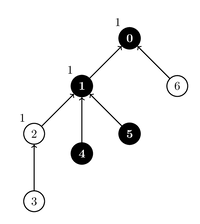
\includegraphics[width=0.26\textwidth]{circuit-way1.png} &
  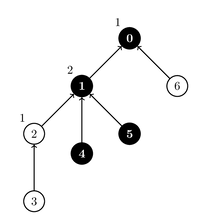
\includegraphics[width=0.26\textwidth]{circuit-way2.png} \\
\end{tabular}
\end{center}

In all other assignments of parameters, gate $0$ has state $0$. Thus, the answer is $2$.

Update $1$ is $L = 4$, $R = 5$. This toggles the states of gates $4$ and $5$. As a result, all source
gates have state $0$, and for any assignment of parameters, gate $0$ has state $0$. Thus, the answer
is $0$.

Update $2$ is $L = 3$, $R = 6$. This changes the states of all source gates to $1$. As a result, for
any assignment of parameters, gate $0$ has state $1$. Thus, the answer is $6$.
